\chapter{Introduzione}

\section{Il Corso in Breve...}

\subsection{Motivazioni}

\dfn{Intelligenza Artificiale}{
  L'intelligenza artficiale (o IA, dalle iniziali delle due parole, in italiano) è una disciplina appartenente all'informatica che studia i fondamenti teorici, le metodologie e le tecniche che consentono la progettazione di sistemi hardware e sistemi di programmi software capaci di fornire all’elaboratore elettronico prestazioni che, a un osservatore comune, sembrerebbero essere di pertinenza esclusiva dell’intelligenza umana.
}

\nt{Meh, in realtà l'IA è una disciplina di confine. Però le tematiche sono prettamente informatiche.}

\paragraph{IA In breve:}

\begin{itemize}
  \item Area di ricerca dell'informatica. 
  \item Si occupa di tutto ciò che serve
per rendere un computer
intelligente come un essere
umano. 
\item Interessata a problemi \fancyglitter{intelligenti}: problemi per cui non esiste/non è noto un algoritmo di risoluzione\footnote{Tris, il labirinto, etc.}.
\end{itemize}

\nt{Il cubo di Rubik non è un gioco intelligente >:(}

\paragraph{Ci sono tante sotto-aree di ricerca:}

\begin{itemize}
  \item Rappresentazione della conoscenza e ragionamento. 
  \item Interpretazione/sintesi del linguaggio naturale. 
  \item Apprendimento automatico. 
  \item Pianificazione. 
  \item Robotica.
\end{itemize}

\paragraph{Si collega a tante discipline, oltre all'informatica:}

\begin{itemize}
  \item Filosofia. 
  \item Fisica. 
  \item Psicologia.
\end{itemize}

\subsubsection{}

Questo insegnamento ha l’obiettivo di approfondire le
conoscenze di Intelligenza Artificiale con particolare riguardo
alle capacità di un agente intelligente di fare \fancyglitter{inferenze} sulla
base di una \fancyglitter{rappresentazione esplicita della conoscenza} sul dominio. In questo corso si faranno anche sperimentazione di metodi di ragionamento basati sul
paradigma della \fancyglitter{programmazione logica}, sull’uso di
\fancyglitter{formalismi a regole} (CLIPS) e su \fancyglitter{reti bayesiane} (ragionamento probabilistico\footnote{Odio la probabilità con tutto il mio cuore <3}).

\paragraph{Programma:}

\begin{itemize}
  \item Dal punto di vista metodologico saranno a rontate problematiche relative a: 
    \begin{itemize}
      \item Meccanismi di ragionamento per calcolo dei predicati del primo
ordine. 
\item Programmazione logica.
\item Ragionamento non monotono. 
\item Answer set programming.
    \end{itemize}
  \item Queste metodologie verranno a rontate dal punto di vista sperimentale con
    l’introduzione dei principali costrutti del \fancyglitter{Prolog}, lo sviluppo di strategie di
ricerca in Prolog e l’utilizzo dell’ambiente \fancyglitter{CLINGO} nella risoluzione di
problemi in cui sia necessaria l’applicazione di meccanismi di ragionamento
non monotono e del paradigma dell’Answer Set Programming.
\end{itemize}


\qs{}{E le novità dell’AI che vanno di moda?}

\paragraph{Risposta:} vengono trattate in altri corsi (TLN, RNDL, AAUT, ELIVA, AGINT).

\section{Il Prolog}

\dfn{Prolog}{
  Prolog (Programming Logic) è un \newfancyglitter{linguaggio dichiarativo} basato sul \newfancyglitter{paradigma logico}: 
  \begin{itemize}
    \item Non si descrive cosa fare per risolvere un problema. 
    \item Si descrive la situazione reale con \newfancyglitter{fatti} e \newfancyglitter{regole} e si chiede all'interprete di verificare se un \newfancyglitter{goal} segue oppure no secondo una logica classica.
  \end{itemize}
}

\nt{Il prolog è equivalente alla logica dei predicati del primordine.}

\subsection{Le Basi}

\dfn{Fatti}{Si rappresenta con dei \newfancyglitter{fatti} un dominio di interesse.}

\ex{Fatto}{
  Fatto per descrivere che un alimento contiene più calorie di un altro: 
  \begin{itemize}
    \item piuCalorico(wurstel, banana). 
    \item Rappresenta il fatto che il würstel è un alimento maggiormente
calorico rispetto alla banana.
  \end{itemize}
}

\dfn{Regole}{
  Si rappresentano le possibili inferenze con delle \newfancyglitter{regole}: 
  \begin{center}
    \texttt{head := subgoal1, subgoal2, \dots, subgoaln}
  \end{center}
}

\ex{Regola}{
  \begin{center}
    \texttt{felino(X) := gatto(X)}
  \end{center}
  Rappresenta la regola che permette di concludere che i gatti sono felini.
}

\paragraph{Idee di base del prolog:}

\begin{itemize}
  \item Regole ricorsive.
  \item L'interprete analizza i fatti e le regole nell'ordine in cui si trovano nel programma. 
  \item Meccanismo di pattern matching per uni care
variabili e termini. 
\item L’interprete, dato un programma, cerca di
dimostrare un goal considerando fatti e applicando
regole, nel secondo caso generando sotto-goal.
\end{itemize}

\dfn{Clausole}{
  Le clausole sono i fatti o le regole. Contengono:
  \begin{itemize}
    \item Atomi: 
      \begin{itemize}
        \item Costanti. 
        \item Numeri.
      \end{itemize}
    \item Variabili.
    \item Termini Composti, ottenuti applicando funtori a termini.

  \end{itemize}
}

\nt{Un programma prolog è un insieme di clausole.}

\clm{}{}{
  \begin{itemize}
    \item L'estensione dei file prolog è 'pl'.
    \item In prolog le variabili hanno l'iniziale maiuscola. 
    \item L'unica struttura dati nativa è la lista.
    \item Per eseguire swi: swipl. 
    \item Per compilare: $[$'nomefile.pl'$]$.
    \item Il comando ';' indica possibili alternative.
    \item Il comando 'trace.' consente un esecuzione passo per passo.
\end{itemize}
}

\dfn{Lista}{
  La \newfancyglitter{lista} è la struttura dati principale in prolog. Una lista è caratterizzata da una testa e da una
coda: 
\begin{itemize}
  \item Testa: primo termine (a sinistra) della lista. 
  \item Coda: la lista dei termini dal secondo (incluso)
in poi.
\end{itemize}
}

\nt{Rappresentata come $[$Head $|$ Tail$]$.}

\begin{figure}[h]
    \centering
    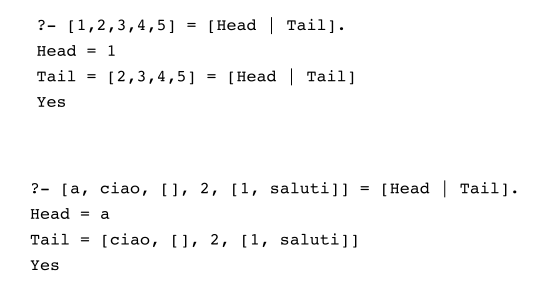
\includegraphics[scale=0.6]{01/liste.png}
    \caption{Le liste in prolog.}
\end{figure}

\paragraph{Predicati \fancyglitter{built-in}:}

\begin{itemize}
  \item \texttt{length(Lista, N)}: ha successo se la \texttt{Lista} contiene \texttt{N} elementi. 
  \item \texttt{member(Elemento,Lista)}: ha successo se la \texttt{Lista} contiene il termine \texttt{Elemento}.
\end{itemize}



